\section*{Abstract}


%Zielsetzung, Problemstellung
An der Hochschule Luzern wurde im Modul Produktentwicklung 2 (PREN 2) ein autonomer Wegfindungsroboter gebaut und getestet. Das Konzept dazu wurde im vorherigen Semester in Produktentwicklung (PREN 1) ausarbeitet. Der Roboter muss in der Lage sein autonom ein linienbasiertes Wegenetz zu durchqueren. Dabei muss er gesperrte Knoten erkennen können, Hindernisse erkennen und versetzen sowie einen zuvor definierten Zielknoten finden. Dabei darf er die Linie des Wegenetzes nie verlassen.


% Methoden
Ausgehend von der Produktbeschreibung aus PREN 1 wuden die einzelen Teilfunktionen des Roboters umgesetzt. Erkenntnisse aus Testaufbauten aus PREN 1 wurden berücksichtigt. Wurde vom ursprünglichen Konzept abgewichen wurde dies begründet. 

\begin{figure}[H]
    \centering
    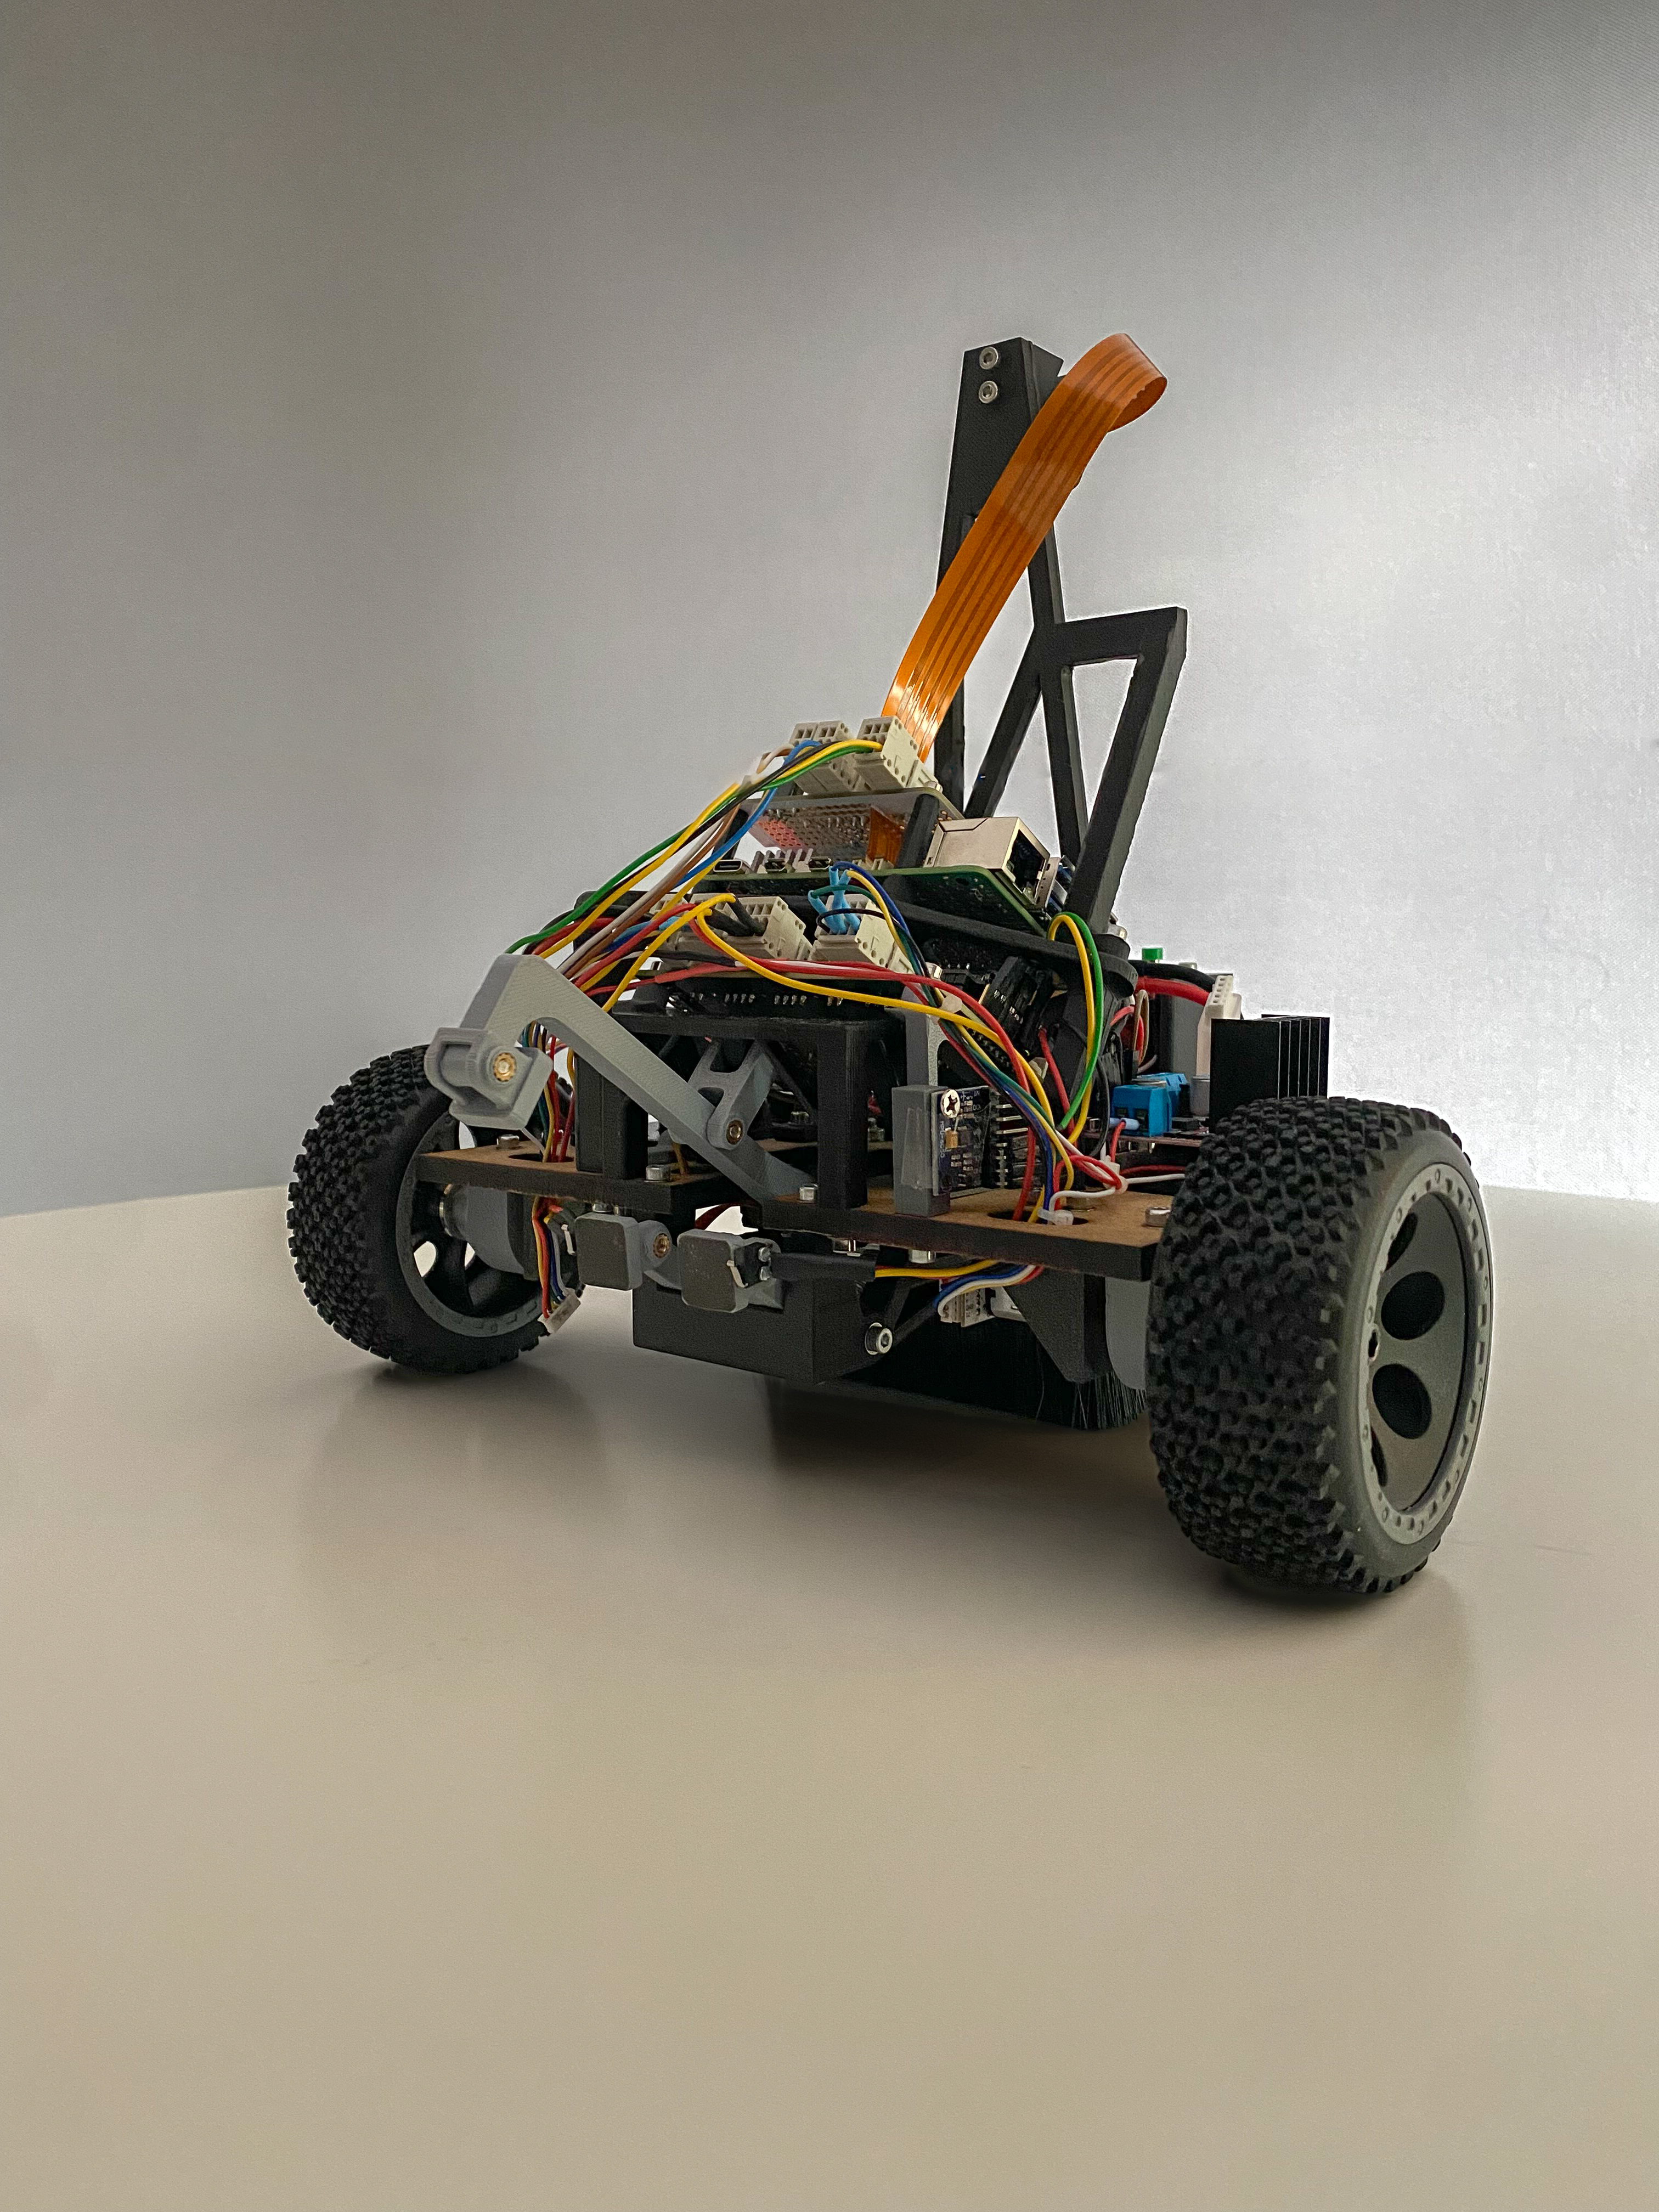
\includegraphics[width=0.4\textwidth, trim={0cm 7cm 0cm 2cm}, clip]{assets/PREN2_Roboter_back.jpg}
    \caption{Rückansicht des Roboters}
    \label{fig:roboter_back}
\end{figure}


% Ergebnissse
Der Roboter, der auf Abbildung \ref{fig:roboter_back} sichtbar ist, fährt mit zwei Motoren mit Encodern und hat vorne ein Stützrad ohne Antrieb. Er folgt der Linie, indem er den untenangebrachten Liniensensor ausliest. Wenn genug Sensoren gleichzeitig eine Linie erkennen, weiss der Roboter, dass er einen Knoten erreicht hat. Auf dem Knoten liest er die ausgehenden Linien, indem er ein Bild mit seiner Kamera davon macht. Danach dreht er sich in die Richtung von jeder Linie und mach ein Bild zu dem nächsten Knoten, dabei wird mit Artificial Intelligence geprüft, ob sich ein Objekt auf der Strecke oder auf dem nächsten Knoten befindet.

Der Roboter wählt die kürzeste, offene Strecke zum Zielpunkt. Falls sich auf dieser eine Barriere befindet, fährt er darauf zu, bis er mit dem Ultraschallsensor merkt, dass sie nah ist, dann dreht er sich 180\textdegree. Er fährt rückwärts, bis seine Endschalter von der Barriere betätigt werden, dann hebt der Greifer, der von einem Servomotor angesteuert wird, das Hindernis auf. Er dreht sich wieder zurück, fährt etwas vor und stellt die Barriere an der gleichen Stelle ab.

Wenn der Roboter denkt, er hat das Ziel erreicht, macht er ein Bild vom Knoten und liest, ob sich auf dem Knoten der richtige Buchstabe befindet. Falls ja, macht er ein Buzzer Geräusch.


% Ausblick
Die einzelnen Teile der Steuerung konnten noch nicht zusammen getestet werden. Jedoch konnten alle Teile alleine getestet werden und die Navigation und die Mechanik konnten jeweils komplett integriert getestet werden. Dies bildet eine gute Grundlage, den Roboter noch bis zum Wettbewerb fahrfähig zu machen.
